\section{終点誤差分散最小モデル}
\textbf{終点誤差分散最小モデル} (minimum-variance model; \cite{Harris1998-gj})を実装する.

$\mathbf{A}\in \mathbb{R}^{n\times n}$, $\mathbf{B}\in \mathbb{R}^{n}$とする.$\dot{x}=\mathbf{A}_{c}\mathbf{x}+\mathbf{B}_{c}(u + w)$について,差分化すると


\begin{align}
\mathbf{x}(t+dt)&=\mathbf{x}(t)+\dot{\mathbf{x}}dt\\
\mathbf{x}_{t+1}&=\mathbf{I}\mathbf{x}_t+(\mathbf{A}_{c}dt)\mathbf{x}_t+(\mathbf{B}_{c}dt)(u + w)
\end{align}


となる(ここで$\mathbf{I}$は単位行列)ので,$\mathbf{A}=\mathbf{I}+\mathbf{A}_{c}dt, \mathbf{B}=\mathbf{B}_cdt$として


\begin{equation}
\mathbf{x}_{t+1} = \mathbf{A} \mathbf{x}_t + \mathbf{B}(u_t + w_t)
\end{equation}


と表せる. $\mathbf{x}_t$の平均は


\begin{equation}
\mathbb{E}\left[\mathbf{x}_{t}\right]=\mathbf{A}^{t} \mathbf{x}_{0}+\sum_{i=0}^{t-1} \mathbf{A}^{t-1-i} \mathbf{B} u_{i}
\end{equation}


$\mathbf{x}_t$の分散は


\begin{equation}
\operatorname{Cov}\left[\mathbf{x}_{t}\right]=k \sum_{i=0}^{t-1}\left(\mathbf{A}^{t-1-i} \mathbf{B}\right)\left(\mathbf{A}^{t-1-i} \mathbf{B}\right)^{\top} u_{i}^{2}
\end{equation}


となる.
\subsection{終点誤差分散最小モデルの実装}
以下では田中先生の\url{https://www.motorcontrol.jp/archives/?MC13}のコードを参考に作成した.
\lstinputlisting[language=julia]{./text/motor-learning/minimum-variance/002.jl}
\lstinputlisting[language=julia]{./text/motor-learning/minimum-variance/003.jl}
\lstinputlisting[language=julia]{./text/motor-learning/minimum-variance/004.jl}
\lstinputlisting[language=julia]{./text/motor-learning/minimum-variance/005.jl}
\lstinputlisting[language=julia]{./text/motor-learning/minimum-variance/006.jl}
結果の描画.
\lstinputlisting[language=julia]{./text/motor-learning/minimum-variance/008.jl}
\begin{figure}[ht]
	\centering
	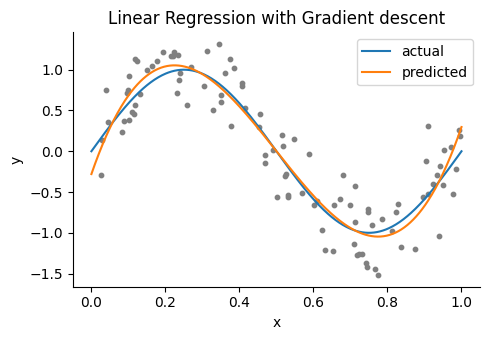
\includegraphics[scale=0.8, max width=\linewidth]{./fig/introduction/linear-regression/cell008.png}
	\caption{cell008.png}
	\label{cell008.png}
\end{figure}
